\documentclass[b5paper,border=10pt]{standalone}
%%%<
\usepackage{verbatim}
%%%>
\usepackage{pgfplots}
\pgfplotsset{width=7cm,compat=1.8}
\begin{comment}
:Title: Surface plot with interior colors
:Tags: 3D;Surface plots;Manual
:Author: Christian Feuersänger
:Slug: surface-interior-color

A surface plot visualizes a two dimensional, single patch using
different fill colors for each patch segment.
Each patch segment is a (pseudo) rectangle, that means input data
is given in form of a data matrix.

We can distinguish between the outer side and the interior
parts of a surface by choosing different colors.

The code is from the PGFPlots 1.10 manual: "4.6.6 Surface Plots".
\end{comment}
\begin{document}
\begin{tikzpicture}[declare function={f(\x)=sqrt(\x);}]
\begin{axis}[small,axis lines=middle,xlabel={$x$},ylabel={$y$},enlargelimits=true,ymax=2.25,xtick={4},ytick={\empty}]
\addplot[domain=0:0.5]{f(x)};
\addplot[domain=0.5:4]{f(x)}node[pos=0.5,above left]{$y=\sqrt{x}$};
\end{axis}
\end{tikzpicture}

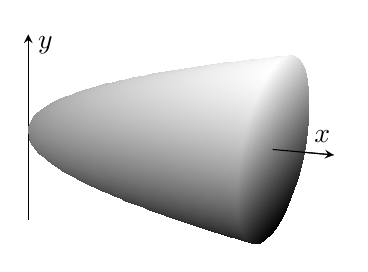
\begin{tikzpicture}
\begin{axis}[small,
  axis lines=center,
axis y line=none,
%  axis on top,
view/h=15,
%view/v=45,
  xlabel={$x$},
% ylabel={$y$},
 zlabel={$y$},
%xlabel style={xshift=1ex},
  domain=0:4,
  y domain=0:2*pi,
  xmin=0, xmax=5,
  ymin=-2.25, ymax=2.25, zmin=-2.25,zmax=2.25,
  %mesh/interior colormap={blueblack}{color=(black) color=(blue)},
  colormap/blackwhite, 
  samples=40,
  samples y=40,
  z buffer=sort,
%shader=flat,
shader=interp,
xtick={\empty}, ytick={\empty},ztick={\empty},
 ]
  \addplot3[surf] ({x},{sqrt(x)*cos(deg(y))},{sqrt(x)*sin(deg(y))});
 \addplot3[surf] ({4},{sqrt(x)*cos(deg(y))},{sqrt(x)*sin(deg(y))});
\draw(axis cs:4,0,0)--(axis cs:5,0,0);
\end{axis}
\end{tikzpicture}
\end{document}
